%%%%%%%%%%%%%%%%%%%%%%%%%%%%%%%%%%%%%%%%%
% a0poster Portrait Poster
% LaTeX Template
% Version 1.0 (22/06/13)
%
% The a0poster class was created by:
% Gerlinde Kettl and Matthias Weiser (tex@kettl.de)
% 
% This template has been downloaded from:
% http://www.LaTeXTemplates.com
%
% License:
% CC BY-NC-SA 3.0 (http://creativecommons.org/licenses/by-nc-sa/3.0/)
%
%%%%%%%%%%%%%%%%%%%%%%%%%%%%%%%%%%%%%%%%%

%----------------------------------------------------------------------------------------
%	PACKAGES AND OTHER DOCUMENT CONFIGURATIONS
%----------------------------------------------------------------------------------------

\documentclass[a0,portrait]{a0poster}

\usepackage{multicol} % This is so we can have multiple columns of text side-by-side
\columnsep=100pt % This is the amount of white space between the columns in the poster
\columnseprule=3pt % This is the thickness of the black line between the columns in the poster

\usepackage[svgnames]{xcolor} % Specify colors by their 'svgnames', for a full list of all colors available see here: http://www.latextemplates.com/svgnames-colors

\usepackage{times} % Use the times font
%\usepackage{palatino} % Uncomment to use the Palatino font

\usepackage{graphicx} % Required for including images
\graphicspath{{figures/}} % Location of the graphics files
\usepackage{booktabs} % Top and bottom rules for table
\usepackage[font=small,labelfont=bf]{caption} % Required for specifying captions to tables and figures
\usepackage{amsfonts, amsmath, amsthm, amssymb} % For math fonts, symbols and environments
\usepackage{wrapfig} % Allows wrapping text around tables and figures
\usepackage{rotating}

\begin{document}

%----------------------------------------------------------------------------------------
%	POSTER HEADER 
%----------------------------------------------------------------------------------------

% The header is divided into two boxes:
% The first is 75% wide and houses the title, subtitle, names, university/organization and contact information
% The second is 25% wide and houses a logo for your university/organization or a photo of you
% The widths of these boxes can be easily edited to accommodate your content as you see fit

\begin{minipage}[b]{0.85\linewidth}
\veryHuge \color{NavyBlue} \textbf{Stellar oscillations induced by a planetary companion} \color{Black}\\ % Title
\Huge\textit{Going off on a tangent}\\[2cm] % Subtitle
\huge \textbf{Andrew Bunting\textsuperscript{1}, John Papaloizou\textsuperscript{2} \& Caroline Terquem\textsuperscript{1}}\\[0.5cm] % Author(s)
\huge \textsuperscript{1}Physics Department, University of Oxford; \textsuperscript{2}DAMPT, University of Cambridge\\[0.4cm] % University/organization
\Large \texttt{andrew.bunting@physics.ox.ac.uk}\\
\end{minipage}
%
\begin{minipage}[b]{0.15\linewidth}

\includegraphics[width=10cm]{ox_logo.png}\\
\end{minipage}

\vspace{1cm} % A bit of extra whitespace between the header and poster content

%----------------------------------------------------------------------------------------

\begin{multicols}{2} % This is how many columns your poster will be broken into, a portrait poster is generally split into 2 columns

%----------------------------------------------------------------------------------------
%	ABSTRACT
%----------------------------------------------------------------------------------------

%\color{Navy} % Navy color for the abstract

%\begin{abstract}

%Sed fringilla tempus hendrerit. Vestibulum ante ipsum primis in faucibus orci luctus et ultrices posuere cubilia Curae; Etiam ut elit sit amet metus lobortis consequat sit amet in libero. Lorem ipsum dolor sit amet, consectetur adipiscing elit. Phasellus vel sem magna. Nunc at convallis urna. isus ante. Pellentesque condimentum dui. Etiam sagittis purus non tellus tempor volutpat. Donec et dui non massa tristique adipiscing. Quisque vestibulum eros eu. Phasellus imperdiet, tortor vitae congue bibendum, felis enim sagittis lorem, et volutpat ante orci sagittis mi. Morbi rutrum laoreet semper. Morbi accumsan enim nec tortor consectetur non commodo nisi sollicitudin. Proin sollicitudin. Pellentesque eget orci eros. Fusce ultricies, tellus et pellentesque fringilla, ante massa luctus libero, quis tristique purus urna nec nibh.

%\end{abstract}

%----------------------------------------------------------------------------------------
%	INTRODUCTION
%----------------------------------------------------------------------------------------

\color{SaddleBrown} % SaddleBrown color for the introduction

\section*{Introduction}

Both the Radial Velocity (RV) and transit methods for detecting exoplanets have been successful, but both are limited -- characterising the planetary system's mass is a particular difficulty due to degeneracy with the inclination or the density, respectively. Understanding other ways in which the planet and the star interact could break these degeneracies.

Given their mass, size and proximity to their host star, Hot Jupiters have a stronger interaction with their host star than other planets. The first-order effect of their presence is what is used to detect them in both the RV and transit method -- the motion of the star around the common centre of mass, and the light blocked by their presence respectively. The tidal potential due to the planet is a second-order effect which changes the amplitude and wavelength of the star's light.

Whilst modelling this interaction for the non-adiabatic case has been undertaken before \cite{Pfahl2008}, a detailed analysis of the tangential displacement has been lacking, or has otherwise been done assuming that the change due to non-adiabaticity is small \cite{Terquem1998}.

This work particularly focusses upon the behaviour at the very surface, where non-adiabatic effects are prominent. Comparison between the modelled behaviour and analytical results under the conditions present at the very surface show good agreement.


%----------------------------------------------------------------------------------------
%	METHOD
%----------------------------------------------------------------------------------------

\color{DarkSlateGray} % DarkSlateGray color for the rest of the content

\section*{Method}

%------------------------------------------------

\subsection*{Numerical method}

To model the oscillations, the linear non-adiabatic stellar oscillation equations were solved in the case that the star is perturbed by a regular tidal potential, due to the planet. The variables directly solved for are: $\xi_{r}$, the radial displacement; $F_{r}'$, the perturbation to the radial radiative flux; $p'$, the perturbation to the pressure; and $T'$, the perturbation to the temperature.

The equations solved are:


\begin{equation} \label{eq:cont_osc}
\frac{1}{r^{2}} \frac{\partial}{\partial r} ( r^{2} \rho_{0} \xi_{r} )  
+ \left( \frac{\rho_{0}}{\chi_{\rho} p_{0}} - \frac{l (l+1)}{m^{2} \omega^{2} r^{2}} \right) p'
- \frac{\rho_{0}}{T_{0}} \frac{\chi_{T}}{\chi_{\rho}} T'
=
\frac{l (l+1)}{m^{2} \omega^{2} r^{2}} \rho_{0} \Phi_{P}
\end{equation}
\\
\begin{equation} \label{eq:ent_osc}
\left( i \rho_{0} m \omega c_{p}  + \frac{l (l+1)}{r^{2}} K_{0} \right) T'
- \left( i m \omega c_{p} \nabla_{ad} \rho_{0} T_{0}  \right) \frac{p'}{p_{0}}
+ i m \omega \rho_{0} T_{0} \frac{\partial s_{0}}{\partial r} \xi_{r}
+ \frac{1}{r^{2}} \frac{\partial}{\partial r} ( r^{2} F_{r}')
=
0
\end{equation}
\\
\begin{multline} \label{eq:flux_osc}
- \frac{F_{r}'}{K_{0}}
+ \left( - \frac{\partial}{\partial r} + \frac{1}{T_{0}} \frac{\partial T_{0}}{\partial r} \left[ -3 + \frac{1}{\kappa_{0}} \left( \frac{\partial \kappa}{\partial \ln T} \right)_{\rho} - \frac{\chi_{T}}{\chi_{\rho}} \left( 1 + \frac{1}{\kappa_{0}} \left( \frac{\partial \kappa}{\partial \ln \rho} \right)_{T} \right) \right] \right) T' \\
+ \frac{\partial T_{0}}{\partial r} \frac{1}{p_{0} \chi_{\rho}} \left( 1 + \frac{1}{\kappa_{0}} \left( \frac{\partial \kappa}{\partial \ln \rho} \right)_{T} \right) p'
=
0
\end{multline}
\\
\begin{equation} \label{eq:mom_osc}
- m^{2} \omega^{2} \rho_{0} \xi_{r} 
+ \left( \frac{\partial}{\partial r} + \frac{\rho_{0}}{\chi_{\rho} p_{0}} \frac{\partial \Phi_{0}}{\partial r} \right) p'
-  \frac{\partial \Phi_{0}}{\partial r} \frac{\rho_{0}}{T_{0}} \frac{\chi_{T}}{\chi_{\rho}} T'
=
- \rho_{0} \frac{\partial \Phi_{P}}{\partial r}
\end{equation}
\\
which correspond to the continuity equation, entropy equation, radiative diffusion equation, and the momentum equation respectively.


The boundary conditions are:

\begin{align}
\xi_{r} &\equiv 0 \text{ at } r = 0 \\
F_{r}' &\equiv 0 \text{ at } r = 0 \\
\Delta p &\equiv  0 \text{ at } r = R \\
4 \frac{\Delta T}{T_{0}} - \frac{\Delta F_{r}}{F_{r_{0}}} &\equiv  0 \text{ at } r = R
\end{align}
\\
which correspond to the displacement and perturbed flux vanishing at the centre to ensure continuity, and the surface boundary conditions ensure that the pressure at the perturbed surface is unchanged, and that the star remains a blackbody.

The Henyey method \cite{Henyey1964} was used to solve these equations, using a solar-type model produced using MESA \cite{Paxton2011} \cite{Paxton2013} \cite{Paxton2015} \cite{Paxton2018} as the equilibrium background star which we perturbed.

%------------------------------------------------

\subsection*{Analytical solution}

For the region at the surface, where $\Delta P \approx 0$, analytical expressions for the relationships between certain variables can be calculated. 





%----------------------------------------------------------------------------------------
%	RESULTS 
%----------------------------------------------------------------------------------------

\section*{Results}

Donec faucibus purus at tortor egestas eu fermentum dolor facilisis. Maecenas tempor dui eu neque fringilla rutrum. Mauris \emph{lobortis} nisl accumsan. Aenean vitae risus ante.
%
\begin{wraptable}{l}{12cm} % Left or right alignment is specified in the first bracket, the width of the table is in the second
\begin{tabular}{l l l}
\toprule
\textbf{Treatments} & \textbf{Response 1} & \textbf{Response 2}\\
\midrule
Treatment 1 & 0.0003262 & 0.562 \\
Treatment 2 & 0.0015681 & 0.910 \\
Treatment 3 & 0.0009271 & 0.296 \\
\bottomrule
\end{tabular}
\captionof{table}{\color{Green} Table caption}
\end{wraptable}
%
Phasellus imperdiet, tortor vitae congue bibendum, felis enim sagittis lorem, et volutpat ante orci sagittis mi. Morbi rutrum laoreet semper. Morbi accumsan enim nec tortor consectetur non commodo nisi sollicitudin. Proin sollicitudin. Pellentesque eget orci eros. Fusce ultricies, tellus et pellentesque fringilla, ante massa luctus libero, quis tristique purus urna nec nibh.

Nulla ut porttitor enim. Suspendisse venenatis dui eget eros gravida tempor. Mauris feugiat elit et augue placerat ultrices. Morbi accumsan enim nec tortor consectetur non commodo. Pellentesque condimentum dui. Etiam sagittis purus non tellus tempor volutpat. Donec et dui non massa tristique adipiscing. Quisque vestibulum eros eu. Phasellus imperdiet, tortor vitae congue bibendum, felis enim sagittis lorem, et volutpat ante orci sagittis mi. Morbi rutrum laoreet semper. Morbi accumsan enim nec tortor consectetur non commodo nisi sollicitudin.

\begin{center}\vspace{1cm}
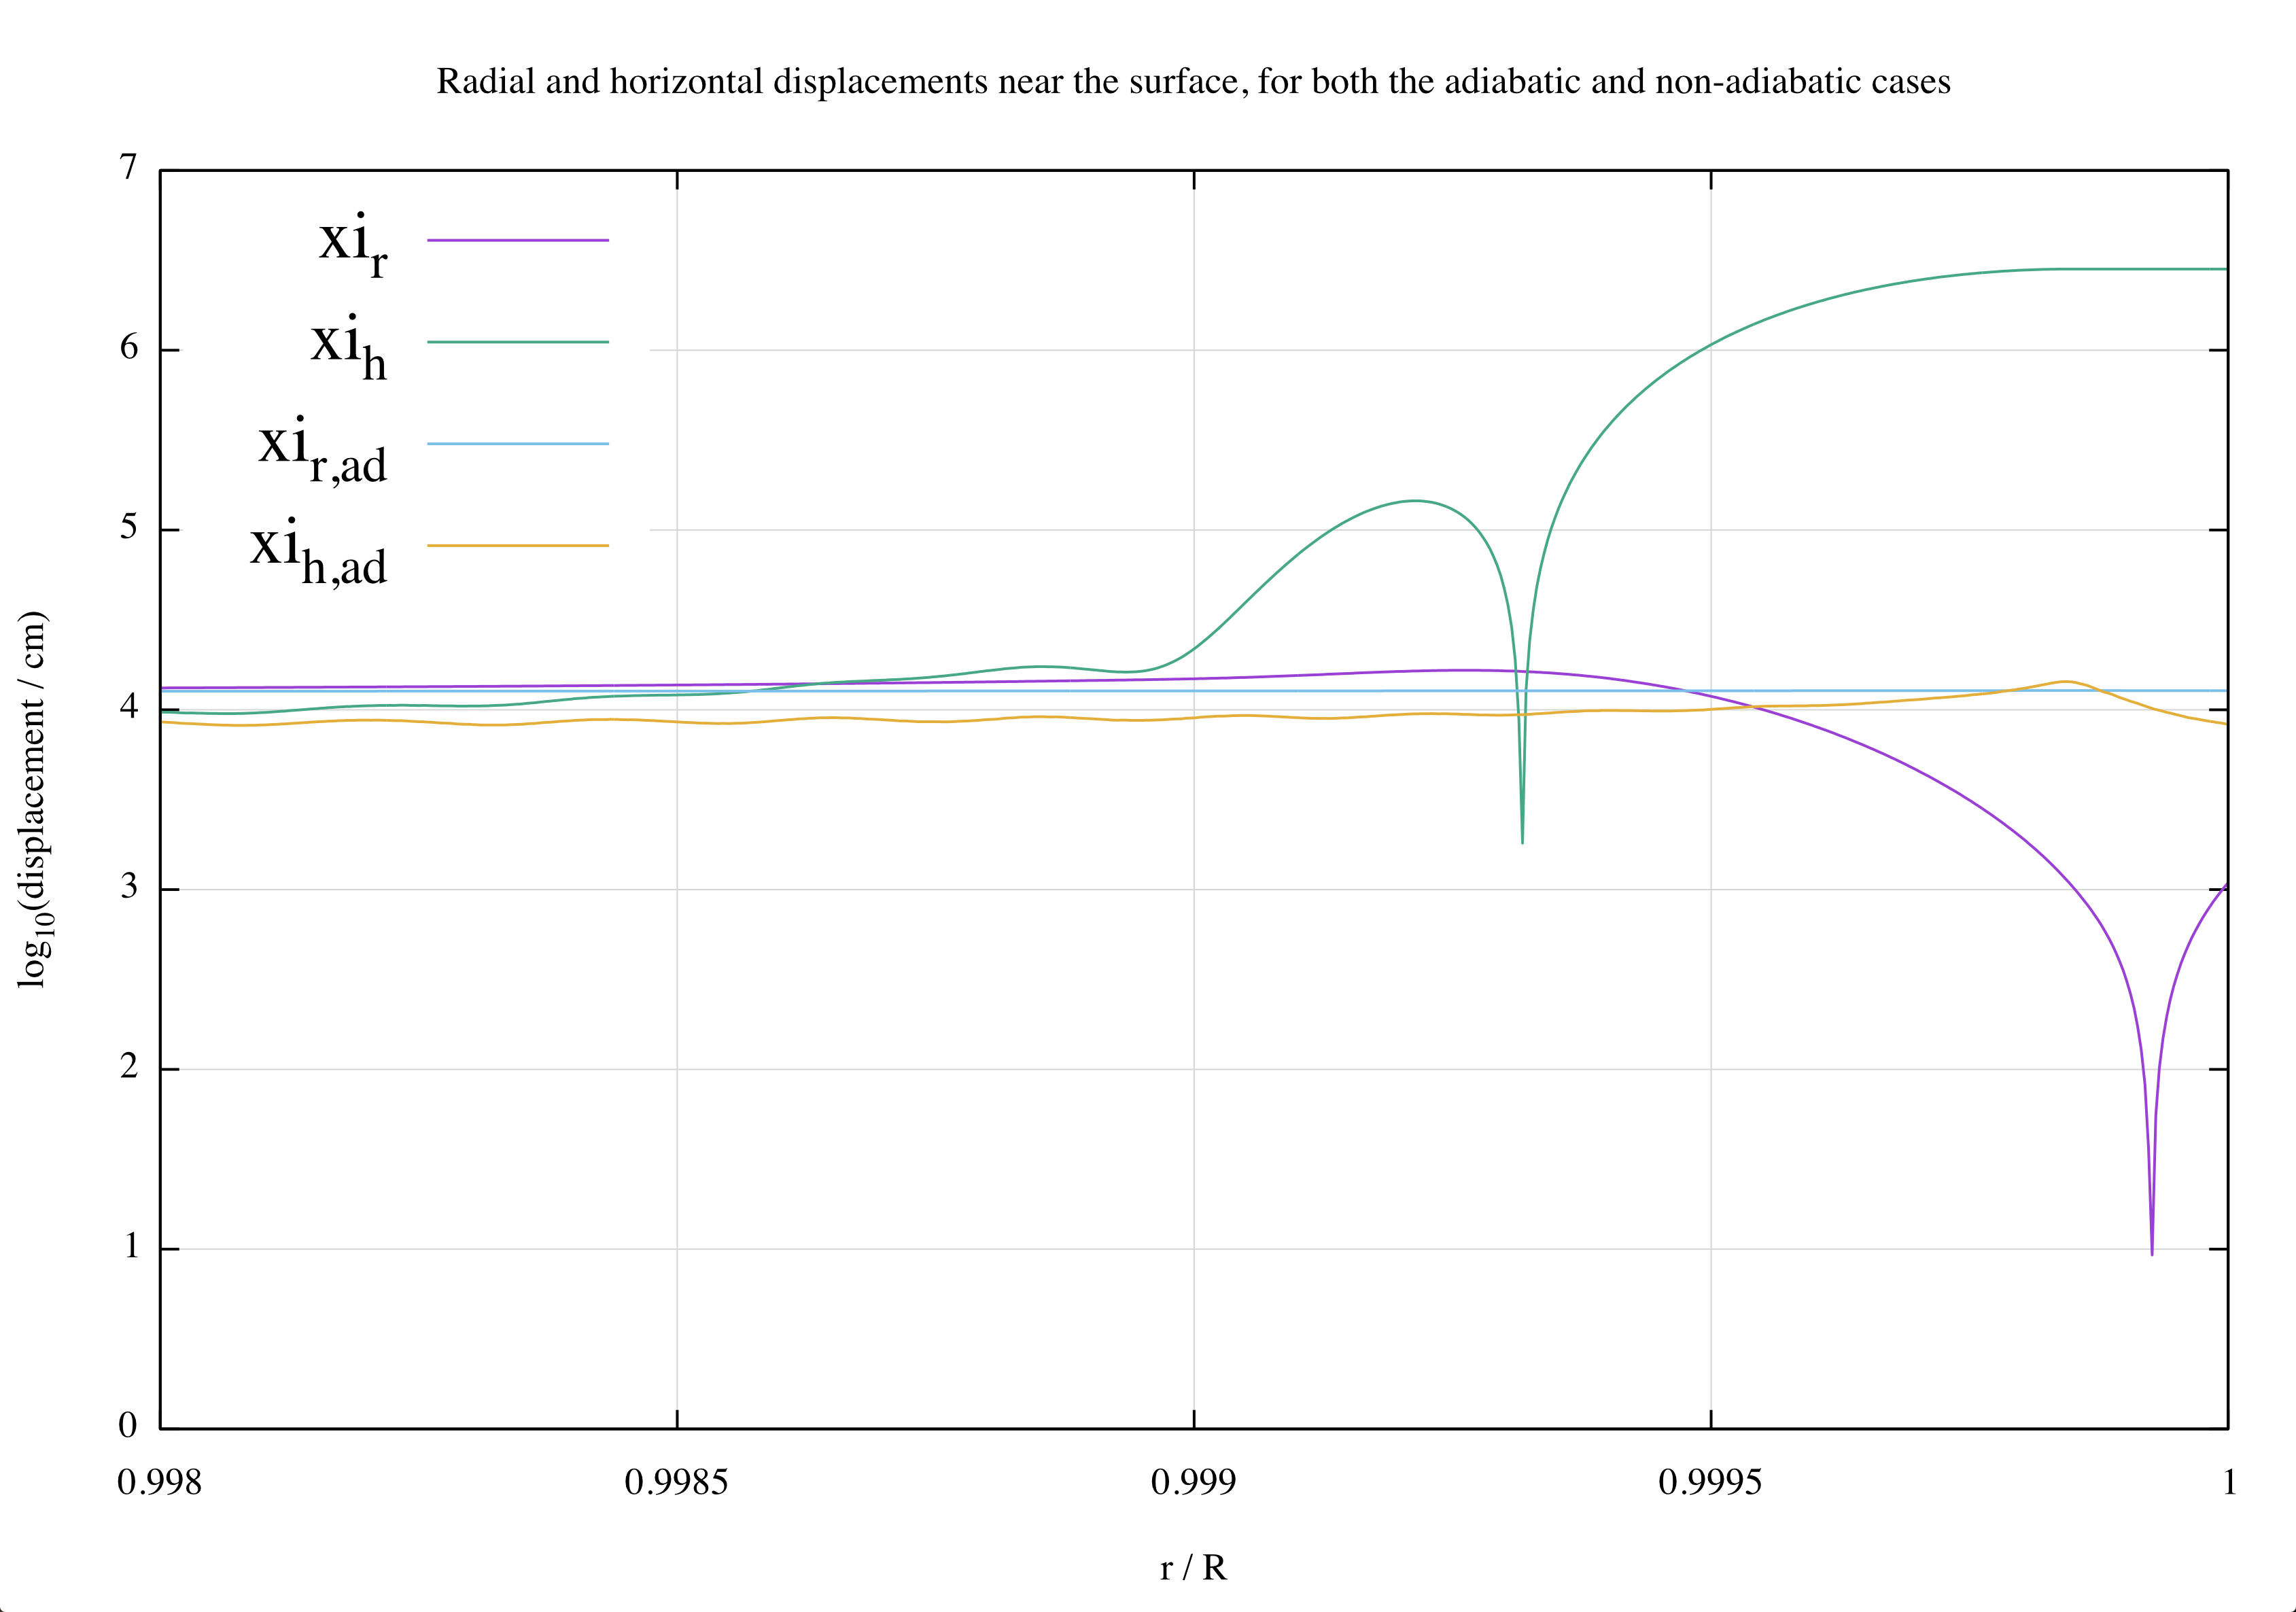
\includegraphics[width=1.0\linewidth]{poster_displacements}
\captionof{figure}{\color{Green} Figure caption}
\end{center}\vspace{1cm}

In hac habitasse platea dictumst. Etiam placerat, risus ac.



Vivamus sed nibh ac metus tristique tristique a vitae ante. Sed lobortis mi ut arcu fringilla et adipiscing ligula rutrum. Aenean turpis velit, placerat eget tincidunt nec, ornare in nisl. In placerat.

\begin{center}\vspace{1cm}
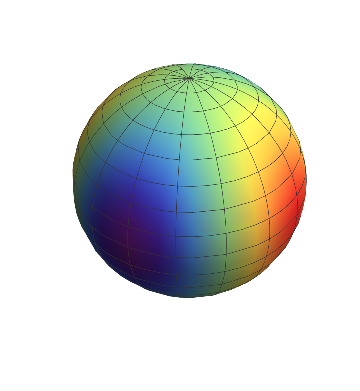
\includegraphics[width=0.45\linewidth]{radial_map}
~
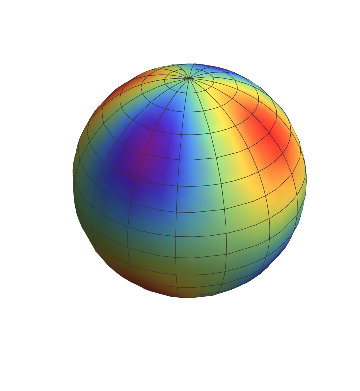
\includegraphics[width=0.45\linewidth]{tangential_map}
\captionof{figure}{\color{Green} Figure caption}
\end{center}\vspace{1cm}

%----------------------------------------------------------------------------------------
%	CONCLUSIONS
%----------------------------------------------------------------------------------------

\color{SaddleBrown} % SaddleBrown color for the conclusions to make them stand out

\section*{Conclusions}

\begin{itemize}
\item Pellentesque eget orci eros. Fusce ultricies, tellus et pellentesque fringilla, ante massa luctus libero, quis tristique purus urna nec nibh. Phasellus fermentum rutrum elementum. Nam quis justo lectus.
\item Vestibulum sem ante, hendrerit a gravida ac, blandit quis magna.
\item Donec sem metus, facilisis at condimentum eget, vehicula ut massa. Morbi consequat, diam sed convallis tincidunt, arcu nunc.
\item Nunc at convallis urna. isus ante. Pellentesque condimentum dui. Etiam sagittis purus non tellus tempor volutpat. Donec et dui non massa tristique adipiscing.
\end{itemize}

\color{DarkSlateGray} % Set the color back to DarkSlateGray for the rest of the content

%----------------------------------------------------------------------------------------
%	FORTHCOMING RESEARCH
%----------------------------------------------------------------------------------------

\section*{Forthcoming Research}

Vivamus molestie, risus tempor vehicula mattis, libero arcu volutpat purus, sed blandit sem nibh eget turpis. Maecenas rutrum dui blandit lorem vulputate gravida. Praesent venenatis mi vel lorem tempor at varius diam sagittis. Nam eu leo id turpis interdum luctus a sed augue. Nam tellus.

 %----------------------------------------------------------------------------------------
%	REFERENCES
%----------------------------------------------------------------------------------------

%\nocite{*} % Print all references regardless of whether they were cited in the poster or not
\bibliographystyle{plain} % Plain referencing style
\bibliography{library} % Use the example bibliography file sample.bib

%----------------------------------------------------------------------------------------
%	ACKNOWLEDGEMENTS
%----------------------------------------------------------------------------------------

\section*{Acknowledgements}

Etiam fermentum, arcu ut gravida fringilla, dolor arcu laoreet justo, ut imperdiet urna arcu a arcu. Donec nec ante a dui tempus consectetur. Cras nisi turpis, dapibus sit amet mattis sed, laoreet.

%----------------------------------------------------------------------------------------

\end{multicols}
\end{document}